\chapter{Revisão Bibliográfica}

A pesquisa bilbliográfica deste trabalho é delineada por: estudo de sistemas
multicorpos, que faz uma revisão da modelagem cinemática e dinâmica desses
sistemas; análise dinâmica de estruturas, que busca métodos para obter a matriz
de rigidez e amortecimento da base; pesquisa sobre manipuladores robóticos
compostos por elementos flexíveis; e tarefas robóticas de precisão \textit{in
situ}.


% -.~.-.~.-.~.-.~.-.~.-.~.-.~.-.~.-.~.-.~.-.~.-
\section{Dinâmica de Sistemas Multicorpos}

A dinâmica de sistemas multicorpos (MBS) é baseada na mecânica clássica. Esses
sistemas são definidos por um ou mais corpos, imperfeitamente conectados, pela
possibilidade de movimento relativo entre eles. A conexão imperfeita de 2 ou
mais corpos rígidos que forma o sistema multicorpo é denominado par cinemático,
ou junta~\cite{de2012kinematic}. Dinâmica multicorpos pode ser entendida como o
estudo de sistemas de vários corpos sujeitos a forças e interações devido a
diferentes tipos de juntas que os conectam e restringem seu
movimento~\cite{flores2008kinematics}, como ilustrado esquematicamente na
Figura~\ref{fig::mbs_diagram}.

\begin{figure}[h]
	\centering 
 	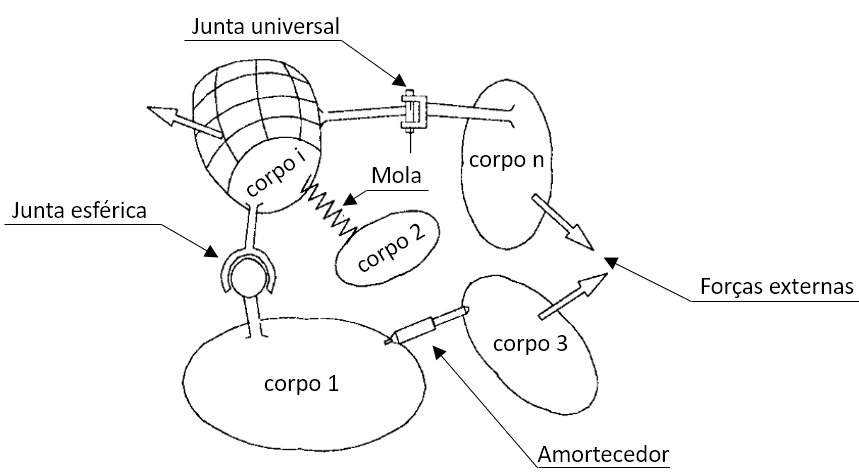
\includegraphics[width=0.75\textwidth]{figs/mbs_diagram}
 	\caption[Representação de um sistema MBS]{Representação de um sistema MBS.
 	\\Fonte: adaptado de \cite{neto2003stabilization}}
 	\label{fig::mbs_diagram}
\end{figure}

A mecânica clássica dos sistemas de corpos rígidos e suas aplicações foram
marcadas por fortes restrições na complexidade dos modelos até a década de 1960.
Entretanto, a necessidade de modelar sistemas mais complexos, como satélites e
veículos espaciais, assim como a rápida evolução dos computadores na época,
abriram caminhos para aplicações mais avançadas de sistemas
multicorpos~\cite{schiehlen1997multibody}.

Hoje, muitos programas estão disponíveis para a modelagem e simulação de
sistemas MBS, e possuem interface gráfica e ferramentas para modelagem ou
importação de corpos CAD e elementos padronizados de conectores, como juntas de
de vários tipos, molas e amortecedores. Para citar alguns:
%
\begin{enumerate*}[label=\roman*]
	\item MSC ADAMS;
	\item Universal Mechanism;
	\item MapleSim.
\end{enumerate*}
%

No entanto, para ter maior controle da modelagem matemática, dos métodos e das
simplificações e tratamento e pós-processamento dos resultados, este trabalho
não fez uso de um programa comercial dedicado. Para isso, derivou-se toda a
cinemática, dinâmica e equações de movimento dos sistemas simbolicamente, no
Sophia-Maple. Isto permite que o método seja livre de qualquer restrição imposta
pelas capacidade de qualquer programa, tornando explícita a metodologia proposta
e permitindo repeti-la e verifica-la em qualquer outra plataforma.


\subsection{Cinemática}\label{sec::cinematica}

Os conceitos de análise cinemática que se seguem nesta seção compõe os
fundamentos básicos de diversos textos de áreas como Dinâmica de Corpos Rígidos,
Sistemas Multicorpos e Robótica. As referências utilizadas para os
fundamentos da cinemática tratados a seguir são:
\cite{tenenbaum2006fundamentals},
\cite{kane1985dynamics},
\cite{shabana2013dynamics},
\cite{sciavicco2012modelling} e
\cite{spong2006robot}

\subsubsection{Sistemas de Coordenadas}

Um corpo rígido é completamente descrito por sua posição e orientação com
respeito a um sistema de coordenadas (SC). Um sistema de coordenadas é um
conjunto de eixos ortogonais que se inteceptam em um ponto, denominado origem.

Geralmente, em sistemas multicorpos, 2 tipos de SC são utilizados. O primeiro é
fixo no tempo e representa uma referência para todos os corpos, denominado
sistema de referência \emph{global} ou \emph{inercial}. O segundo tipo é
solidário a cada componente do sistema, representando um SC \emph{local}, que
translada e gira com o corpo. A Figura~\ref{fig::sist_refs} apresenta um corpo
B, seu referencial local SC-B e um referncial inercial SC-R, que descrevem o mesmo
ponto $p$ em B, por 2 vetores diferentes.

\begin{figure}[h]
	\centering 
 	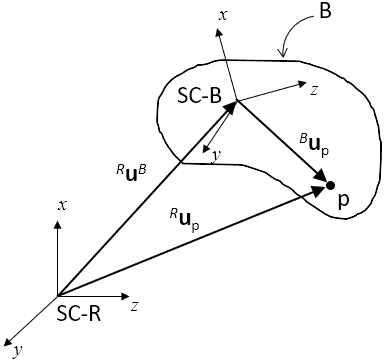
\includegraphics[width=0.45\textwidth]{figs/sist_refs}
 	\caption{Sistemas de referência global e local}
 	\label{fig::sist_refs}
\end{figure}

Os vetores que descrevem a posição do ponto $p$ em cada referencial podem ser
definidos com 3 coordenadas:
%
\begin{align}
	^{R}\textrm{\textbf{u}}_{p} = [r1, r2, r3]^{R} \\
	^{B}\textrm{\textbf{u}}_{p} = [b1, b2, b3]^{B}
\end{align}
%
Note-se que $^{R}\textrm{\textbf{u}}_{p}$ também pode ser escrito como a soma de
2 vetores:
%
\begin{equation}
	^{R}\textrm{\textbf{u}}_{p} = {}^{R}\textrm{\textbf{u}}^{B} + 
	{}^{B}\textrm{\textbf{u}}_{p}
\end{equation}
%

Logo, qualquer ponto no do corpo B pode ser descrito como uma soma da posição
do referencial do corpo, com respeito ao referencial global, mais o vetor posição
do ponto com respeito ao refencial local.

A escolha dos SC's impacta substancialmente no tamanho das equações
cinemáticas que descrevem os movimentos dos corpos. Uma escolha perspicaz do conjunto de
SC's utilizado é importante para a eficiência do código e do cálculo
computacional.

\subsubsection{Matrizes de Rotação e Transformação Homogênea}

As matrizes de rotação definem a orientação relativa entre 2 sistemas de
coordenadas. As matrizes que representam as rotações básicas em torno
dos eixos $x, y$ e $z$ são: 
%
\begin{equation}
	R_{x,\theta} = 
\begin{pmatrix}
1 &0  &0 \\ 
0 &\cos(\theta)  &-\sin(\theta) \\ 
0 &\sin(\theta)  &\cos(\theta) 
\end{pmatrix}
\end{equation}
%
\begin{equation}
R_{y,\theta} = 
\begin{pmatrix}
\cos(\theta) &0  &\sin(\theta) \\ 
0 &1  &0 \\ 
-\sin(\theta) &0  &\cos(\theta) 
\end{pmatrix}
\end{equation}
%
\begin{equation}
R_{z,\theta} = 
\begin{pmatrix}
\cos(\theta) &-\sin(\theta)  &0 \\ 
\sin(\theta) &\cos(\theta)  &0 \\ 
0 &0  &1
\end{pmatrix}
\end{equation}
%

Uma matriz rotação geral $R$, pode ser definida pela sequência ilimitada de
quaisquer rotações básicas. Por exemplo:
%
\begin{equation}
	R_{ZYZ} = R_{z,\phi} \cdot R_{y,\theta} \cdot R_{z,\psi}
\end{equation}
%
Esta em especial representa um método comum para para especificar a matriz de
rotação que orienta um corpo em função 3 quantidades independentes $\phi, \theta, \psi$,
denominado \emph{Ângulos de Euler}, tal que de 3 rotações, não
ocorram 2 rotações sucessivas em torno do mesmo eixo.
Outros métodos comuns para especificar uma matriz de rotação são ângulos \textit{Roll-Pitch-Yaw}, ângulos de Bryan e
representação Eixo-Ângulo.

Se os referenciais são coincidentes, a representação de um vetor com respeito a
outro referencial é simplesmente a projeção do vetor através da matriz de
rotação:
%
\begin{equation}
^{A}\textrm{\textbf{p}} = R_{B}^{A} \cdot {}^{B}\textrm{\textbf{p}}
\end{equation}
%

Se um referencial fixo num corpo desloca-se em relação a outro referencial, como
na Figura~\ref{fig::sist_refs}, a representação de $p$ descrito em SC-R, pode
ser torna-se:
%
\begin{equation} \label{eq::upemr}
	^{R}\textrm{\textbf{u}}_{p} = {}^{R}\textrm{\textbf{u}}^{B} + R \cdot
	{}^{B}\textrm{\textbf{u}}_{p}
\end{equation}
%

Uma forma mais prática de representar o deslocamento geral dos corpos do sistema
(rotação e translação) ao longo de diferentes referenciais é utilizando o
conceito de matrizes de Transformação Homogênea. É basicamente uma representação
do movimento rígido na forma matricial. 
\begin{equation}
	H = 
\begin{pmatrix}
R & d\\ 
0 & 1
\end{pmatrix} ~,~ \in ~ \mathbb{R}_{4\times4}
\end{equation}
%
Onde $R$ representa a matriz de rotação $3\times3$ e $d$ o vetor translação
$3\times1$ entre os referenciais.

Logo, a equação~\ref{eq::upemr}, poderia ser representada simplesmente por:
%
\begin{equation}
	^{R}\textrm{\textbf{u}}_{p} = H_{B}^{R} \cdot ^{B}\textrm{\textbf{u}}_{p}
\end{equation}

\subsubsection{Velocidade Angular, Linear e Aceleração}

Assumindo que um referencial associado a um corpo C se move em relação
um referencial R, então há um vetor $^{R}\boldsymbol{\omega}^{C}$ tal que para
todo vetor $\mathbf{v}$ fixo em $C$, sua derivada temporal em relação ao
referencial $R$ é:
%
\begin{equation}
	\frac{\mathrm{d} \mathbf{v}}{\mathrm{d} t} = {}^{R}\boldsymbol{\omega}^{C}
	\times \mathbf{v}
\end{equation}
%
Onde o vetor ${}^{R}\boldsymbol{\omega}^{C}$ é chamada vetor velocidade angular
de C em R.
De uma forma mais geral, a relação de um vetor $\mathbf{u}$, com respeito a 2
referenciais, movendo-se arbitrariamente em relação um ao outro é expresso como:
%
\begin{equation} \label{eq::velgeral}
	\frac{^{A}\mathrm{d} \mathbf{u}}{\mathrm{d} t} = \frac{^{B}\mathrm{d}
	\mathbf{u}}{\mathrm{d} t} + {}^{A}\boldsymbol{\omega}^{B} \times \mathbf{u}
\end{equation}
%
A equação~\ref{eq::velgeral} define a velocidade do vetor $\mathbf{u}$ com
respeito ao referencial A. Portanto, do sistema genérico da
Figura~\ref{fig::sist_refs}, pode-se escrever a velocidade do ponto $p$ como:
%
\begin{equation}
	^{R}\mathbf{v}^{p} = {}^{B}\mathbf{v}^{p} + ^{R}\mathbf{v}^{B} +
	{}^{A}\boldsymbol{\omega}^{B} \times {}^{B}\textrm{\textbf{u}}_{p}
\end{equation}
%

A aceleração do ponto $p$ com respeito ao referencial R será a derivada temporal
da velocidade com respeito a R. Logo:
%
\begin{equation}
	^{R}\mathbf{a}^{p} = \frac{^{A}\mathrm{d} }{\mathrm{d} x} {^{R}\mathbf{v}^{p}}
\end{equation}
%
Fazendo-se a derivada temporal, obtém-se a expressão:
%
\begin{equation}
	^{R}\mathbf{a}^{p} = {}^{B}\mathbf{a}^{p} + {}^{R}\mathbf{a}^{B} +
	{}^{R}\boldsymbol{\omega}^{B} \times ({}^{R}\boldsymbol{\omega}^{B} \times
	{}^{B}\mathbf{u}_p) + {}^{R}\boldsymbol{\alpha}^{B} \times {}^{B}\mathbf{u}_p
	+ 2{}^{R}\boldsymbol{\omega}^{B} \times {}^{B}\mathbf{v}^{p}
\end{equation}
%
Onde ${}^{R}\boldsymbol{\alpha}^{B}$ é o vetor aceleração angular do referencial
B em relação a R e o termo $2{}^{R}\boldsymbol{\omega}^{B} \times
{}^{B}\mathbf{v}^{p}$ é o chamado \emph{aceleração de Coriolis}. 


\subsubsection{Cinemática de Manipuladores Robóticos}

Manipuladores robóticos consistem em um sistema mecânico composto por uma série
de corpos(elos), conectados por juntas. Cada junta fornece um, e apenas um, grau
de liberdade, podendo ser translacional (primsático) ou rotacional (juntas de
revolução). A estrutura de juntas de um robô pode ser descrita por uma sequência
de caracteres representando os tipos de juntas: ``R'' para rotacional e ``P''
para prismática. Logo, o manipulador MOTOMAN MH12 pode ser caracterizado por
RRRRRR, por exemplo, por possuir 6 juntas de revolução.

A formulação das relações cinemáticas permitem o estudo de um problema chave em
robótica, da cinemática direta, que consiste na determinação de um método
sistemático e geral para descrever o movimento do efetuador, em função do
movimento das juntas.

Um método largamente utilizado para sistematização da análise cinemática de
manipuladores robóticos, é de \emph{Denavit-Hartenberg} (DH).
Consiste em definir as matrizes de transformação homogênea de cada elo $i$ a
partir de apenas 4 parâmetros: $\theta_i, a_i, d_i, \alpha_i$, que são
respectivamente comprimento, torção e \textit{offset} do elo, e ângulo da junta.

A cinemática direta, portanto, envolve o cálculo da pose (posição e orientação)
do efetuador, $\xi_{E}$, como função do valor da juntas $\mathbf{q}$. 
%
\begin{equation}
	\xi_{E} = \mathcal{K}(\mathbf{q})
\end{equation}
%


\subsection{Cinemática Inversa}\label{sec::ikin}

O problema inverso, ou seja, encontrar o valor das juntas $\mathbf{q}$ que
satisfazem $\xi_{E}$ é feito pela análise da cinemática inversa. Logo:
%
\begin{equation} \label{eq::invq}
	\mathbf{q} = \mathcal{K}^{-1}(\xi_{E})
\end{equation}
%

A solução deste problema é fundamental importância, porque transforma o
movimento desejado do efetuador, no espaço cartesiano, no valor correspondente
das juntas. Entretanto, o problema da cinemática inversa é muito mais complexo,
pelos seguintes motivos:
%
\begin{itemize}
  \item As equações a serem resolvidas são geralmente não lineares, então nem
  sempre é possível obter uma solução de forma fechada;
  \item Múltiplas ou infitas soluções podem existir;
  \item Dependendo da estrutura cinemática do manipulador, pode não existir
  solução admissível.
\end{itemize}
%

\subsubsection{Desacoplamento cinemático}

De qualquer forma, para o manipulador de 6 gdl MOTOMAN MH12 que é tratado nesta
pesquisa, há pelo menos 16 soluções admissíveis, número que é reduzido se
considerados os limites de juntas.

A maioria dos manipuladores atuais são cinematicamente simples, e é devido a
dificuldade da solução da cinemática inversa que eles evoluiram assim. Há hoje
diversas técnicas para resolver o problema, para citar alguns exemplos: método
analítico, geométrico, subproblemas de Paden-Kahen, Jacobiano Transposto,
Pseudoinversa e Mínimos Quadrados Amortecido~\cite{buss2004introduction}. 

Devido a sua simplicidade, e por funcnionar bem com a modelagem simbólica
no Sophia-Maple, o método utilizado foi o geométrico. É demonstrado a seguir a
metodologia apresentada por \citet{spong2006robot} para chegar à solução da
equação~\ref{eq::invq} pela abordagem geométrica.

O manipulador MOTOMAN MH12 possui 6 graus de liberdade e é caracterizado como um
manipulador antropomórfico com pulso esférico. Assim, as 3 primeiras juntas são
consideradas apenas para posicionamento, e as 3 últimas para orientação do
efetuador. Se as juntas de orientação podem ser modeladas como coincidentes, e
tratá-las como um pulso esférico, este tipo de manipulador permite desacoplar
o problema em 2 subproblemas:
cinemática inversa de posição e cinemática inversa de orientação. A
Figura~\ref{fig::decoupling} ilustra o conceito de desacoplamento, onde
$\mathbf{p}_W$ refere-se a posição da origem do pulso, $\mathbf{p}_E$ a posição
do efetuador e $\mathbf{d}_E$ a distância do efetuador para o pulso.

\begin{figure}[h]
	\centering 
 	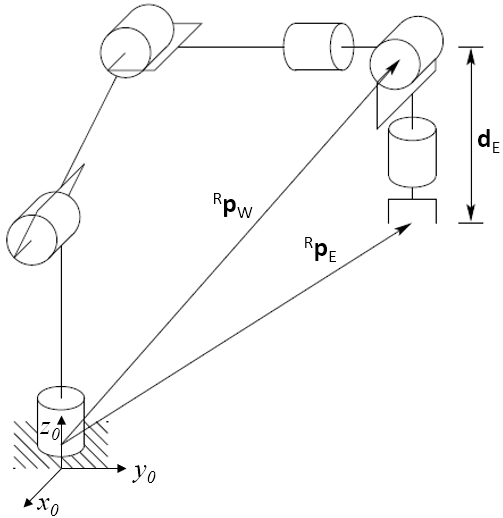
\includegraphics[width=0.45\textwidth]{figs/decoupling}
 	\caption[Desacoplamento cinemático]{Desacoplamento cinemático \\ Fonte:
 	adaptado de~\cite{spong2006robot}}
 	\label{fig::decoupling}
\end{figure}

\subsubsection{Solução da cinemática inversa de posicionamento}

Considerando-se apenas as 3 primeiras juntas do manipulador, pode-se fazer a
análise geométrica das Figuras~\ref{fig::geom_pos_sup} e
\ref{fig::geom_pos_lat} para verificar as seguintes relações:
%
\begin{align}
	\theta_{1} &= \atantwo(x_c, y_c) \pm \atantwo(-\sqrt{r^2-d^2}, -d)
	\label{eq::theta1}\\
	\theta_{2} &= \atantwo(\sqrt{x_c^2+y_c^2-d^2}, z_c-d_1) - \atantwo(a_2+a_3
	c_3,a_3 s_3) \\
	\theta_{3} &= \atantwo(D, \pm \sqrt{1-D^2}) \label{eq::theta2}
\end{align}
%
\begin{equation*}
		D = \frac{x_c^2+y_c^2-d^2 + (z_c-d_1)^2 - a_2^2 - a_3^2}{2a_2 a_3}
\end{equation*}
%
Onde $(x_c, y_c, z_c)$ é a posição da extremidade do manipulador em que
é acoplado o pulso, $d$ é a distância de \textit{offset} da primeira junta,
$a_2$ e $a_3$ são os comprimentos dos elos. Utiliza-se a notação simplificada
das funções trigonométricas, portanto $s_2, c_2$, por exemplo, correpondem a
$\sin(\theta_2)$ e $\cos(\theta_2)$ respectivamente.


\begin{figure}[h]
	\centering 
 	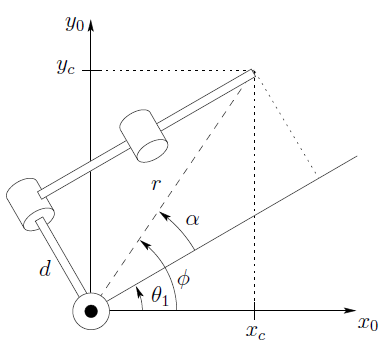
\includegraphics[width=0.45\textwidth]{figs/geom_pos_sup}
 	\caption[Vista na projeção xy do manipulador]{Vista na projeção xy do manipulador
 	\\ Fonte: adaptado de~\cite{spong2006robot}}
 	\label{fig::geom_pos_sup}
\end{figure}

\begin{figure}[h]
	\centering 
 	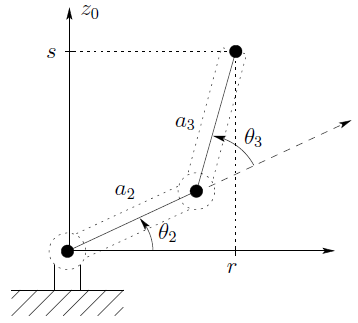
\includegraphics[width=0.45\textwidth]{figs/geom_pos_lat}
 	\caption[Vista na projeção xz do manipulador]{Vista na projeção xz do
 	manipulador \\ Fonte: adaptado de~\cite{spong2006robot}}
 	\label{fig::geom_pos_lat}
\end{figure}

Note-se que as equações encontradas fornecem 4 soluções de configuração do
manipulador para um mesmo ponto no espaço.

Para corresponder ao manipulador MOTOMAN MH12, as equações~\ref{eq::theta1} a
\ref{eq::theta2} sofrem pequenas modificações, que serão detalhadas
posteriormente.

\subsubsection{Solução da cinemática inversa de orientação}

O problema da orientação inversa corresponde a encontrar os valores das 3 jnutas
do pulso para determinar a orientação desejada. A orientação desejada pode ser
definida pelos ângulos de Euler $\phi, \theta, \psi$ que transformam a
orientação do referencial inercial para a orientação final do referencial do
efetuador.
Então, basta encontrar os ângulos $\theta_4, \theta_5, \theta_6$ que satisfazem
a orientação desejada.

Logo, a equação que deve ser resolvida é a seguinte:
%
\begin{equation}
	R_3^6 = (R_0^3)^T R
\end{equation}


A matriz $R$ é a que define a orientação desejada. Utilizando os ângulos de
Euler para rotações em torno dos eixos YZY é:
%
\begin{equation}
R_{YZY} = 
\left( \begin {array}{ccc} c_\phi \,c_\theta \,c_\psi -s_\phi \,s_\psi &-c
\phi \,s_\theta &c_\phi \,c_\theta \,s_\psi +s_\phi \,c_\psi 
\\ \noalign{\medskip}s_\theta \,c_\psi &c_\theta &s_\theta \,s_\psi 
\\ \noalign{\medskip}-s_\phi \,c_\theta \,c_\psi -c_\phi \,s_\psi &s_\phi \,
s_\theta &-s_\phi \,c_\theta \,s_\psi +c_\phi \,c_\psi \end {array} \right)
\end{equation}
%

A matriz de rotação da transformação homogênea entre o referencial inercial e o
referencial do pulso é:
%
\begin{equation}
	(R_0^3)^T = 
\begin{pmatrix}
c_1 c_{23} & -c_1 s_{23}  & s_1 \\ 
s_1 c{23} & -s_1 s_{23}  & -c_1 \\ 
s_{23} & c_{23}  & 0 
\end{pmatrix}
\end{equation}
%
E do pulso para o efetuador:
%
\begin{equation}
R_3^6 = 
\left( \begin {array}{ccc} { c_4}\,{ c_5}\,{ c_6}-{ s_4}\,{
 s_6}&-{ c_4}\,{ s_5}&{ c_4}\,{ c_5}\,{ s_6}+{ c_6}\,{
 s_4}\\ \noalign{\medskip}{ s_5}\,{ c_6}&{ c_5}&{ s_5}\,{
 s_6}\\ \noalign{\medskip}-{ c_5}\,{ c_6}\,{ s_4}-{ c_4}\,{
 s_6}&{ s_4}\,{ s_5}&-{ c_5}\,{ s_4}\,{ s_6}+{ c_4}\,{
 c_6}\end {array} \right)
\end{equation}
%

Logo, utilizando os resultados da cinemática inversa de posicionamento,
$\theta_1, \theta_2, \theta_3$ e definindo-se a orientação pelos ângulos de
Euler $\phi, \theta, \psi$ estão fornecidas no total 9 equações para 3
incógnitas $\theta_4, \theta_5, \theta_6$. 

\subsection{ Planejamento de trajetória} \label{sec::plan_traj}










% exact cellular de composition
% Bountrophedon Path
% Coverage path planning

Os parâmetros como posição, velocidade e orientação ao longo de um dado caminho
são impostos ao robô através do planejamento da trajetória.

% O planejamento é feito aliando-se o caminho desejado aos requisitos necessários
% ligados a uma deter

A importância de incluir corretamente os parâmetros da trajetória se
deve ao fato de que são estes parâmetros que serão verificados ao se comparar
os resultados do robô no modelo de base rígida aos resultados do modelo do robô
sobre uma base flexível. 

Se a tarefa é, por exemplo, o processo de revestimento por HVOF de uma
superfície , o robô deve seguir uma trajetória ao longo daquela superfície, de
forma a cobrí-la totalmente com o material aspersado. Como visto na
seção~\ref{sec::ikin_traj} uma maneira simples de cobrir uma superfície é pelo
movimento de ``zigue-zague'', ilustrado
na Figura~\ref{fig::zigzag}.\todo{Rever / reescrever esse parágrafo}

\missingfigure{Figura esquemática da trajetória}.

O sistema de revestimento por HVOF que motiva este trabalho, realiza a tarefa
sobre uma superfície suavemente curva, que representa o perfil hidráulico, da pá
da turbina. Como um dos requisitos do processo é manter a distância fixa entre a
pistola de revestimento e a pá, a trajetória não está restrita a apenas um
plano.

\begin{figure}[h]
	\centering 
 	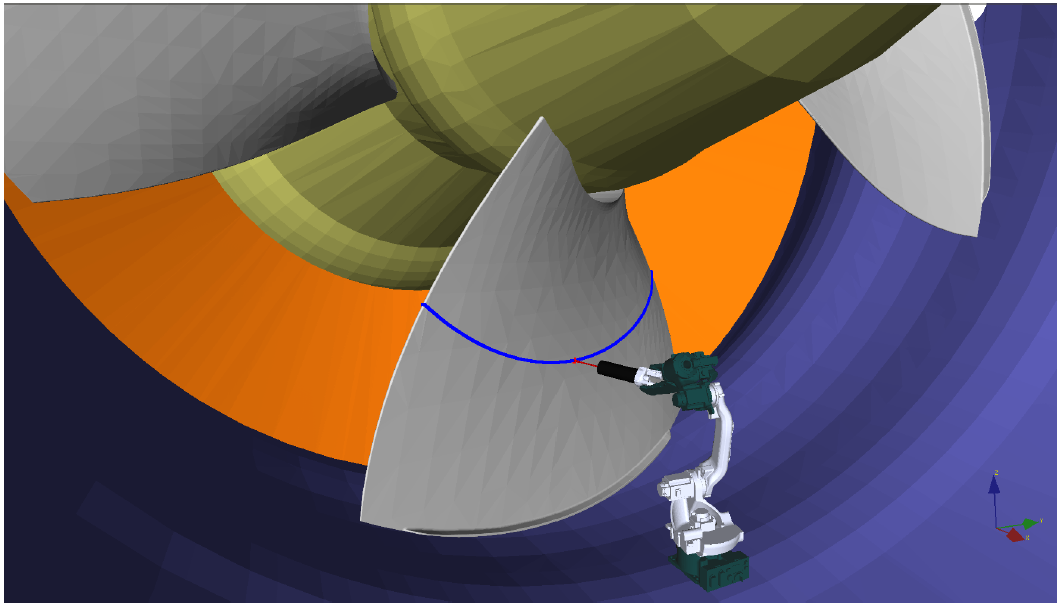
\includegraphics[width=0.75\textwidth]{figs/coat_blade}
 	\caption[Revestimento da face curva de uma pá]{Revestimento da face curva de
 	uma pá. \\Fonte: \citet{8206216}}
 	\label{fig::trajec_600x30}
\end{figure}

\subsection{Dinâmica e Equações de Movimento}

\subsubsection{Equações de Newton-Euler}

% The dynamics of multibody systems is based on classical mechanics. The most
% simple element of a multibody system is a free particle which can be treated by
% Newton’s equations published in 1686 in his “Philosophiae Naturalis Principia
% Mathematica” [111]. The principal element, the rigid body, was introduced in 1775
% by Euler in his contribution entitled “Nova methodus motum corporum rigidarum
% determinandi” [43]. For the modeling of constraints and joints, Euler already used
% the free body principle resulting in reaction forces. The equations obtained are
% known in multibody dynamics as Newton–Euler equations.  ``Schielen, p.149''

\subsubsection{Princípio de d'Alembert}

% A system of constrained rigid bodies was considered in 1743 by d’Alembert in his
% “Trait´e de Dynamique” [32] where he distinguished between applied and reaction
% forces. D’Alembert called the reaction forces “lost forces” having the principle
% of virtual work in mind. A mathematical consistent formulation of d’Alembert’s
% principle is due to Lagrange [89] combining d’Alembert’s fundamental idea with
% the principle of virtual work. As a result a minimal set of ordinary
% differential equations (ODE) of second order is found. ``Schielen, p.150''


\subsubsection{Equações de Lagrange}

% A systematic analysis of constrained mechanical systems was established in
% 1788 by Lagrange [89], too. The variational principle applied to the total kinetic
% and potential energy of the system considering its kinematical constraints and the
% corresponding generalized coordinates result in the Lagrangian equations of the
% first and the second kind. Lagrange’s equations of the first kind represent a set of
% differential-algebraical equations (DAE) while the second kind leads to a minimal
% set of ordinary differential equations (ODE). ``Schielen, p.150''

\subsection{Sophia-Maple e Método de Kane}\label{sec::sophia-kane}

\subsubsection{Notação de Lesser e Lennartsson}


% -.~.-.~.-.~.-.~.-.~.-.~.-.~.-.~.-.~.-.~.-.~.-
\section{Análise dinâmica de estruturas}

\subsection{Matriz de rigidez} \label{sec::rigidez}

\subsection{Amortecimento proporcional} \label{sec::amortecimento}

\subsection{Frequência Natural, Modo de Vibração e Amortecimento}
\label{sec::param_mod}

\subsection{Ensaio experimental de vibrações}


% -.~.-.~.-.~.-.~.-.~.-.~.-.~.-.~.-.~.-.~.-.~.-
\section{Manipuladores robóticos industriais}\label{sec::manind}

\subsection{Manipuladores flexíveis}

\subsection{Manipuladores sobre bases flexíveis}

\subsection{Tarefas de precisão utilizando manipuladores robóticos}

\subsection{Sistema de revestimento por asperção térmica} \label{sec::hvof}

\subsection{Tarefas robóticas \textit{in-situ}} \label{sec::insitu}



\begin{figure}[h]
	\centering 
 	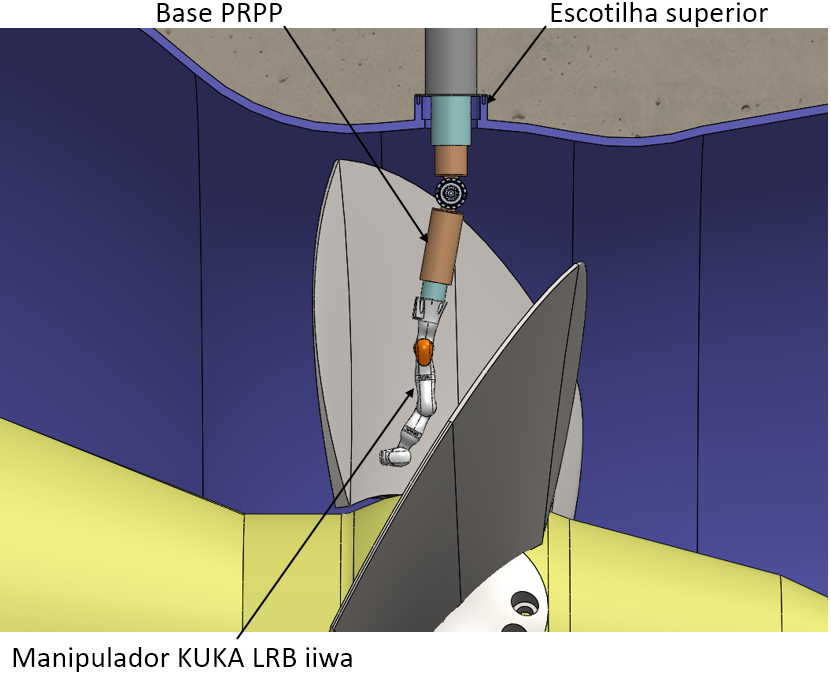
\includegraphics[width=0.85\textwidth]{figs/base_telesc_turbina}
 	\caption{Base telescópica PRPP para manutenção de revestimento
 	\textit{in-situ}}
 	\label{fig::base_telesc_turbina}
\end{figure}

\begin{figure}[h]
	\centering 
 	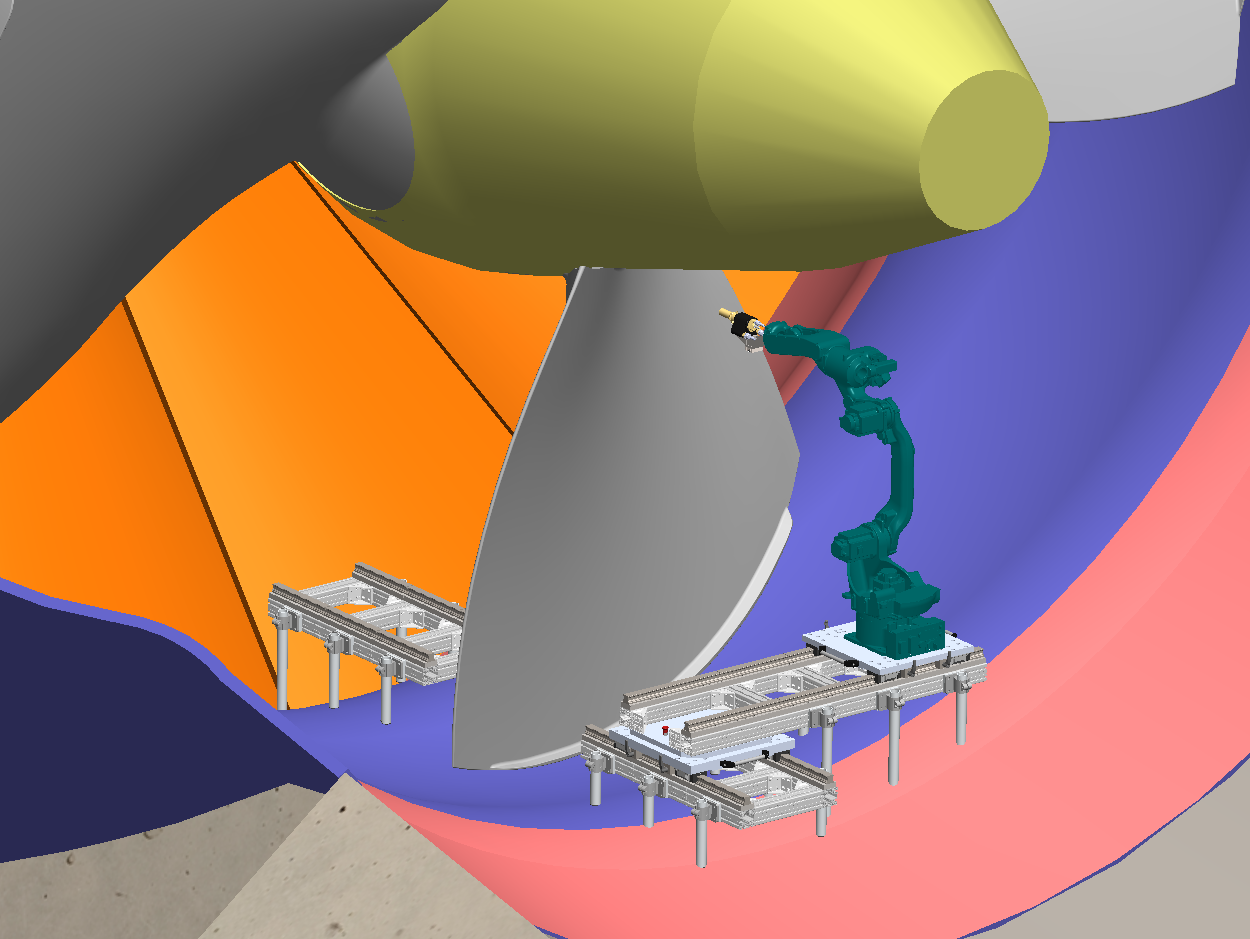
\includegraphics[width=0.85\textwidth]{figs/prp_turbina}
 	\caption{Base modular PRP para manutenção de revestimento \textit{in-situ}}
 	\label{fig::prp_turbina}
\end{figure}




















